\documentclass[conference]{IEEEtran}

\usepackage[utf8]{inputenc}
\usepackage[T1]{fontenc}
\usepackage{hyperref}
\usepackage{url}
\usepackage{booktabs}
\usepackage{amsmath}
\usepackage{amsfonts}
\usepackage{nicefrac}
\usepackage{microtype}
\usepackage{xcolor}
\usepackage{tikz}
\usepackage{graphicx}
\usetikzlibrary{positioning, arrows.meta, shapes.geometric, calc, backgrounds}

\title{Fairness-Aware Online Learning Under Concept Drift}

\author{%
  Tiago Silva\thanks{Corresponding author} \\
  Department of Informatics Engineering\\
  University of Coimbra\\
  \texttt{tds@student.uc.pt} \\
}

\begin{document}

\maketitle

\begin{abstract}
\end{abstract}

\section{Introduction}
The increasing deployment of machine learning (ML) systems in high-stakes decision-making domains, including healthcare~\cite{8474918}, criminal justice~\cite{10467221}, 
and hiring~\cite{10.1145/3351095.3372828}, where their predictions may directly affect individuals and society makes optimizing for performance an insufficient objective; 
models must also satisfy fairness requirements to ensure equitable treatment across individuals or groups of individuals~\cite{10.1145/3457607}. In this regard,  
among the fairness literature, \emph{group fairness}~\cite{10.1145/2090236.2090255} has emerged as one of the most widely studied paradigms, aiming to ensure that predictive behaviour is
balanced across populations defined by sensitive attributes such as gender, race, or age. Common formulations include demographic parity, equal 
opportunity, and equalized odds, each imposing statistical constraints on model outcomes across groups (sometimes mutual incompatible)~\cite{10.1145/2090236.2090255,NIPS2016_6a9659fe}.
Most existing fairness-aware models, however, are developed under the assumption of a stationary data distribution. In practice, 
real-world environments are inherently dynamic, and the statistical properties of data may evolve over time due to policy changes, behavioural 
shifts, seasonal effects, economic fluctuations, or other social transformations. This phenomenon, commonly referred to as concept drift, 
occurs when the relationship between input variables and target outcomes changes over time, causing previously learned decision boundaries to 
become outdated. Different forms of concept drift~\cite{DBLP:journals/corr/WebbHCNP15} change how models must react and adapt. Such changes can significantly degrade 
predictive performance if models are not robust enough to adapt to new patterns. More critically, concept drift also poses a significant threat to the fairness of ML systems. As data distributions shift, 
the statistical relationships that underpin fairness guarantees may also change, potentially leading to increased bias and unfair treatment of certain groups.
To address this challenge, the online learning and data stream mining literature has proposed numerous adaptive methods capable of detecting and 
responding to concept drift in real time. These approaches often rely on drift detection mechanisms combined with incremental learning 
strategies to maintain predictive accuracy under non-stationary conditions. Nevertheless, the majority of existing methods focus primarily on 
predictive utility, while fairness considerations remain comparatively underexplored. As a result, fairness guarantees established during training 
may deteriorate over time even when predictive accuracy remains relatively stable. This limitation is particularly critical in high-stakes applications, 
where persistent fairness violations may remain undetected for extended periods, compromising trustworthiness, reinforcing societal inequalities, 
and causing tangible harm to affected groups.
Existing fairness-aware online learning methods remain limited along two main axes. First, many approaches that explicitly handle drift focus exclusively on predictive
performance, leaving fairness guarantees unmonitored once the underlying distribution moves. Second, methods that do enforce fairness in streaming settings typically rely on
static interventions—fixed regularizers, fixed thresholds, or one-shot pre-processing—that adapt slowly, if at all, to shifts in the protected-attribute conditional or the
decision boundary. These limitations highlight an important gap in the literature and motivate the following research questions:
\begin{itemize}
\item \textbf{RQ1:} To what extent does concept drift affect group fairness metrics in online learning settings?
\item \textbf{RQ2:} Can adaptive drift detection and response mechanisms preserve fairness guarantees while maintaining predictive performance over time?
\item \textbf{RQ3:} How do different types of concept drift influence the stability and robustness of fairness-aware learning models?
\end{itemize}
Based on these research questions, this work investigates fairness-aware online learning under concept drift. We introduce \textsc{FADO} (Fairness-Aware Drift-aware Online learning),
a framework that wraps an existing fair oblique decision forest—\textsc{Aranyani}~\cite{chowdhury2024enhancing}—with a dual-threshold drift detector and a reaction controller that
modulates the optimizer learning rate and the soft-routing temperature in response to detected change. We emphasize that \textsc{Aranyani} is not contributed by this paper:
it serves as the in-processing base learner around which \textsc{FADO} builds its drift-detection and response machinery. Our central hypothesis is that fairness degradation under
concept drift can be mitigated by coupling an in-processing fairness-aware ensemble with an explicit, fairness-aware adaptive controller, allowing the model to maintain both
predictive utility and equitable treatment across demographic groups in non-stationary environments.

To evaluate this hypothesis, we run a prequential, test-then-train evaluation on three standard fairness benchmarks: the \textsc{Adult} income dataset, the \textsc{COMPAS} recidivism
dataset, and the \textsc{Folktables} (ACS Income, CA) dataset; on \textsc{Adult} we additionally inject four controlled synthetic drift scenarios that isolate distinct dimensions of
distributional change, while \textsc{Folktables} provides a natural cross-year shift between 2015 and 2017--2018. \textsc{FADO} is compared against three streaming baselines covering
the accuracy/fairness/adaptivity design space: \textsc{ARF}~\cite{10.1007/s10994-017-5642-8}, an accuracy-oriented Adaptive Random Forest with drift detection but no fairness mechanism;
\textsc{RFR}, a sharpness-aware fairness-reweighted variant without adaptive drift handling; and \textsc{FERMI}~\cite{lowy2021fermi}, a fair logistic-regression baseline based on an
exponential R\'enyi mutual-information regularizer. The experimental results demonstrate that pairing a fairness-aware ensemble with an explicit reaction controller substantially
improves fairness stability over time while maintaining competitive predictive performance, and that fairness degradation is highly sensitive to the nature and intensity of the
drift, reinforcing the importance of adaptive fairness-aware mechanisms in dynamic environments. The main contributions of this work are:
\begin{itemize}
\item \textsc{FADO}, a fairness-aware online learning framework that wraps a fair oblique decision forest with a dual-threshold ADWIN drift detector and a reaction controller acting on the learning rate and the soft-routing temperature;
\item An empirical analysis, across four synthetic drift scenarios on \textsc{Adult} and one natural cross-year shift on \textsc{Folktables}, of how different forms of concept drift affect group fairness metrics over time;
\item A comparison against three streaming baselines (\textsc{ARF}, \textsc{RFR}, \textsc{FERMI}) showing that adaptive fairness mechanisms can preserve fairness guarantees while maintaining predictive performance in non-stationary environments.
\end{itemize}
The remainder of this paper is organized as follows: Section~2 reviews the literature on fairness-aware machine learning and concept drift adaptation; Section~3 defines the 
problem statement, notation, fairness metrics, online evaluation, and drift; Section~4 describes the methodology and experimental design; Section~5 discusses results; and 
Section~6 concludes and outlines directions for future work.

\section{Related Work}
Most existing work on fair machine learning algorithms can be grouped into three categories: (i) pre-processing methods, (ii) in-processing and (iii) post-processing methods.
This is the most common taxonomy used in the literature and it helps providing a clear overview of the different approaches commonly used to achieve fairness. 
\subsection{Pre-processing methods}
Pre-processing methods aim to mitigate bias in the data before the training stage of a model. Xiong et al.~\cite{Xiong_Dalmasso_Mishler_Potluru_Balch_Veloso_2024} 
propose leveraging training samples reweighting to satisfy demographic parity while minimizing distributional distortion using Wasserstein distance to the original dataset. Although
effective, this method does not account for concept drift, nor proves robustness to other forms of fairness violations which limits its applicability in dynamic environments.
Zeng et al.~\cite{zeng2024fairrrpreprocessinggroupfairness} propose a different approach that contrasts with the aforementioned, modifying the actual data labels by treating the 
removal of discrimination from the training dataset as a randomized response problem. The main contribution of this work is the provision 
of a theoretical bridge between pre-processing and techniques to downstream Bayes-optimal classifiers and the fact that it is model agnostic: because it only alters 
the training labels, users do not need to modify their current pipelines. However, this method also does not account for concept drift nor it's impact, and it is limited 
by the binary setup, meaning it only works with binary sensitive attributes and binary outcomes.
\subsection{In-processing methods}
In-processing methods incorporate fairness constraints directly into the learning algorithm. Because our work falls in this category, 
we focus on approaches that strongly inspired our method.

FERMI~\cite{lowy2021fermi} formulates fairness as minimizing the statistical dependence between predictions and sensitive attributes using an exponential Rényi 
mutual information regularizer, which yields a differentiable objective compatible with stochastic optimization and provides theoretical guarantees for common group 
fairness notions such as demographic parity and equalized odds.

Chowdhury et al.~\cite{chowdhury2024enhancing} propose Aranyani, an online fair-learning framework based on ensembles of soft-routed oblique decision trees. 
Unlike standard axis-aligned trees, oblique trees employ learned linear combinations of features at internal nodes, enabling more expressive decision boundaries. 
The ensemble structure further improves predictive robustness by aggregating predictions from multiple trees, reducing variance and preventing overfitting.
A key contribution of Aranyani is the enforcement of fairness constraints at the level of individual tree nodes rather than only at the final output layer. 
The method focuses on statistical parity (demographic parity), introducing node-level fairness constraints that induce parameter isolation, meaning that each 
fairness constraint depends only on local node parameters instead of the entire model. This property substantially improves optimization tractability and empirically 
yields better fairness--accuracy trade-offs.

The framework is specifically designed for online learning scenarios where data arrive sequentially. Traditional in-processing fairness approaches often become 
computationally expensive in streaming environments because fairness objectives depend on group-level expectations over historical data. To address this issue, 
Aranyani maintains running aggregate statistics for each protected group and uses these summaries to estimate fairness gradients efficiently without storing past samples. 
This enables memory-efficient and computationally practical fairness-aware online learning.
The paper additionally provides theoretical analysis of the optimization procedure and evaluates the method on multiple benchmark datasets spanning vision and language tasks, 
demonstrating competitive fairness--accuracy trade-offs relative to baseline approaches. However, the current implementation only supports demographic parity and binary 
protected attributes, and it does not explicitly address concept drift or non-stationary data distributions. Furthermore, many reported baselines are modified variants of the 
proposed method rather than fundamentally different adaptive approaches. These limitations motivate our work, which extends fairness-aware online ensembles with robust adaptive 
mechanisms for non-stationary environments.


While Aranyani focuses primarily on fairness-aware optimization in online learning, another closely related line of work addresses adaptation under concept drift. 
Gomes et al.~\cite{10.1007/s10994-017-5642-8} propose Adaptive Random Forest (ARF), a streaming ensemble framework designed for evolving data distributions. 
ARF extends classical random forests to streaming settings by combining online bagging, randomized feature selection, and adaptive drift detection mechanisms. 
The framework employs ensembles of Hoeffding Trees trained incrementally on sequential data streams and uses Poisson-based online bagging to efficiently simulate bootstrap 
resampling in a single-pass setting.

A major contribution of ARF is its explicit handling of concept drift. Each tree in the ensemble is equipped with independent warning and drift detectors. 
When a warning signal is triggered, a background tree starts training in parallel using incoming data. If drift is later confirmed, the original tree is replaced with the 
partially trained background model, enabling rapid recovery from abrupt or gradual distributional changes without retraining the entire ensemble from scratch. The independence 
of ensemble members also allows efficient parallelization and scalability for high-throughput streams.
Experimental results on synthetic and real-world benchmarks demonstrate strong predictive performance and robustness across various drift scenarios, including abrupt, gradual, 
and incremental concept drift. Consequently, ARF has become a widely adopted benchmark in data stream mining literature. However, despite its strong adaptive capabilities, 
ARF is designed exclusively for predictive adaptation and does not incorporate fairness constraints or bias mitigation mechanisms. As a result, fairness properties may 
deteriorate significantly under distributional shifts, motivating the need for fairness-aware adaptive streaming methods such as the one proposed in this work. We will 
later prove that the our method strongly outperforms ARF in terms of both fairness and performance under drift. 

Some approaches have already attempted to handle drift in fairness-aware settings. Jiang et al.~\cite{jiang2023chasingfairnessdistributionshift} study the problem of 
maintaining fairness under distribution shift. They assume that distribution shift can be modeled as an equivalent perturbation in the parameter space of the learned model. 
Based on this assumption, they propose a robust fairness regularization method that optimizes for worst-case performance under bounded model weight perturbations, improving 
fairness robustness under unseen shifts.
\subsection{Post-processing methods}
Post-processing methods adjust model predictions after training to accomplish fairness objectives. Unlike pre-processing and in-processing approaches, 
these methods do not require modifying the original training data or retraining the underlying model. Instead, fairness is enforced by transforming the model outputs, 
such as prediction labels, confidence scores, or decision thresholds. This makes post-processing particularly attractive in high-stakes domains where predictive systems 
are proprietary, computationally expensive to retrain, or inaccessible to practitioners.

One of the most influential post-processing approaches was introduced by Hardt et al.~\cite{hardt2016equalityopportunitysupervisedlearning}, who proposed a framework for enforcing equalized odds and 
equality of opportunity through randomized threshold adjustments. The method computes group-specific decision rules that probabilistically alter classifier outputs to 
equalize error rates across demographic groups. Because the optimization is performed after model training, the approach is model-agnostic and can be applied to arbitrary 
black-box classifiers. The framework has become a foundational baseline in fairness-aware machine learning due to its simplicity and strong theoretical guarantees. However, 
the method may substantially alter calibration properties and often introduces discontinuities in prediction behavior caused by fixed randomization regions.

Building upon this line of work, Mishler et al.~\cite{Mishler_2021} propose a post-processing framework for achieving counterfactual equalized odds in 
risk assessment instruments. The authors argue that standard fairness notions based on observable outcomes can be inappropriate in intervention settings where observed labels are themselves 
influenced by prior decisions or treatments. To address this issue, the method reformulates 
equalized odds using potential outcomes from causal inference, enforcing fairness with respect to counterfactual outcomes rather than observed ones. Experimental results on COMPAS 
recidivism prediction and child welfare screening demonstrate that the approach can substantially reduce fairness violations with relatively small predictive performance 
degradation. Nevertheless, the method relies on strong causal assumptions, including no unmeasured confounding and positivity, which may be difficult to verify in real-world 
deployments.

More recently, Small et al.~\cite{Small_2024} revisit equalized odds post-processing from the perspective of individual fairness. The authors observe that traditional 
randomized thresholding approaches can treat highly similar individuals differently despite satisfying group-level fairness constraints. In particular, fixed randomization 
intervals may produce discontinuous prediction probabilities, violating the principle that similar individuals should receive similar outcomes. To address this limitation, 
the paper introduces preferential randomization, a continuous post-processing strategy based on smooth monotonic probability curves. Empirical evaluations on credit scoring and recidivism 
prediction tasks demonstrate that the method achieves comparable group fairness and predictive accuracy while significantly improving consistency between similar individuals. 
However, despite these improvements, the framework still operates purely at the prediction layer and does not explicitly address fairness degradation under concept drift or 
evolving data distributions.

Notwithstanding the significant contributions of these post-processing methods to the fairness literature, they are primarily developed under static data assumptions and are, therefore,
not currently focused on addressing the challenges posed by concept drift in online learning settings. As a result, while they may effectively mitigate bias at a given point in time, their fairness guarantees may deteriorate as data distributions evolve.

\subsection{Main Limitations of Prior Work}
\label{sec:related:limitations}
Synthesising the three families surveyed above, we identify four recurring limitations that jointly motivate this work and the design of \textsc{FADO}:
\begin{itemize}
  \item \textbf{L1 -- Static fairness assumption.} The majority of pre-, in-, and post-processing methods are developed under a stationary-data assumption. Once the protected-attribute conditional or the label distribution shifts, the fairness guarantees obtained at training time provide no protection at deployment.
  \item \textbf{L2 -- Adaptive methods are accuracy-oriented.} Streaming ensembles such as \textsc{ARF}~\cite{10.1007/s10994-017-5642-8} explicitly detect and react to drift but do so purely on the predictive-error signal, with no mechanism for tracking or correcting fairness violations.
  \item \textbf{L3 -- Existing fair online learners do not react to drift.} \textsc{Aranyani}~\cite{chowdhury2024enhancing} and \textsc{FERMI}~\cite{lowy2021fermi} provide memory-efficient online fairness, but their regularisers are non-adaptive: when the distribution moves they continue to optimise the same penalty with the same hyperparameters, and convergence to the new optimum is slow.
  \item \textbf{L4 -- Drift-aware fair methods rely on assumptions that do not transfer to streams.} Approaches such as~\cite{jiang2023chasingfairnessdistributionshift} treat distribution shift as a bounded weight-space perturbation, which is informative for worst-case analysis but does not yield an actionable online detector or controller.
\end{itemize}
\textsc{FADO} addresses L1--L4 directly by retaining the node-level fairness regulariser of \textsc{Aranyani} as the in-processing base learner, and adding on top of it (i) an ADWIN-based dual-threshold detector on the online error stream, (ii) a reaction controller that modulates the optimiser learning rate and the soft-routing temperature on warning and confirmation events, and (iii) a rolling-window fairness monitor whose statistics also drive the fairness-aware updates.

\section{Problem Statement}
\subsection{Online Learning Setting}
We consider an online binary classification problem over a data stream $\{(x_t, y_t, a_t)\}_{t=1}^{T}$, where $x_t \in \mathbb{R}^d$ is the feature vector observed at time $t$,
$y_t \in \{0,1\}$ is the binary target label, and $a_t \in \mathcal{A}$ is a sensitive attribute taking values in a finite set with $|\mathcal{A}|=K \ge 2$. Following the
formulation of previous work~\cite{chowdhury2024enhancing,ijcai2019p205}, at each time step the learner receives $x_t$, produces a prediction
$\hat{y}_t = \arg\max f_t(x_t)$, then observes $(y_t, a_t)$ and updates its parameters under a prequential, test-then-train protocol. The fairness formulation introduced below
supports arbitrary $K$, although some datasets are binarised in our study.

\subsection{Group Fairness Metrics}
We focus on \emph{group fairness}, which assesses whether model behaviour is statistically similar across protected groups. Let $\mathcal{A}_t \subseteq \mathcal{A}$ denote the set
of sensitive groups observed within the current evaluation window, and let $\hat{p}_a = \mathbb{E}[\hat{y} \mid a]$ be the positive-prediction rate for group $a \in \mathcal{A}_t$.
We define the unweighted mean group rate as
\[
\bar{p} = \frac{1}{|\mathcal{A}_t|}\sum_{a' \in \mathcal{A}_t}\hat{p}_{a'},
\]
i.e.\ the average positive-prediction rate across the observed groups (a reference value against which each per-group rate $\hat{p}_a$ is compared). The \emph{demographic parity
(DP) violation} is then the worst-case deviation of any group's positive-prediction rate from this mean,
\[
\mathrm{DP} = \max_{a \in \mathcal{A}_t}\left|\hat{p}_a - \bar{p}\right|,
\]
and is bounded between $0$ (perfect parity) and $1$ (one group always predicted positive while another never is). DP measures bias in the prediction \emph{marginal} and is
sensitive to differences in base rates across groups.

To complement DP we also report \emph{equalised odds} (EO), a label-conditional notion of fairness that compares group prediction rates separately within each true-label
class. For each $y \in \{0,1\}$,
\[
\hat{p}_{a|y} = \mathbb{E}[\hat{y} \mid a, y], \qquad
\bar{p}_y = \frac{1}{|\mathcal{A}_t|}\sum_{a' \in \mathcal{A}_t}\hat{p}_{a'|y},
\]
where $\hat{p}_{a|y}$ is the positive-prediction rate of group $a$ \emph{within} class $y$ and $\bar{p}_y$ is the corresponding cross-group mean (the natural per-class
analogue of $\bar{p}$). The EO violation is then
\[
\mathrm{EO} = \max_{y \in \{0,1\}} \max_{a \in \mathcal{A}_t}
\left|\hat{p}_{a|y} - \bar{p}_y\right|,
\]
i.e.\ the worst-case group deviation across both classes; restricting the outer maximisation to $y=1$ yields equal opportunity, which captures bias in the true-positive
rate only. EO is particularly informative when base rates differ across groups, because it disentangles bias from class imbalance.

\subsection{Node-Level Fairness Regulariser}
To connect these group-level fairness notions with the learning objective, we follow the in-processing strategy introduced
by~\cite{chowdhury2024enhancing} and impose fairness constraints on the local outputs of the soft-routed oblique trees that form the base learner of \textsc{FADO}. Let
$n_{ij}(x)\in[0,1]$ denote the soft routing decision at node $(i,j)$, where $i$ indexes the depth and $j$ the node within that depth, i.e.\ the probability with which an
input $x$ is routed to the right child of that node. Each node thus plays a role analogous to a per-step prediction, and the same group-fairness language can be applied to it.
For demographic parity, define
\[
\bar{n}_{ij,a} = \mathbb{E}[n_{ij}(x) \mid a], \qquad
\bar{n}_{ij} = \frac{1}{|\mathcal{A}|}\sum_{a' \in \mathcal{A}} \bar{n}_{ij,a'},
\]
where $\bar{n}_{ij,a}$ is the group-conditional average routing decision at node $(i,j)$ (the analogue of $\hat{p}_a$ but applied to the routing signal) and $\bar{n}_{ij}$ is its
unweighted cross-group mean. The \emph{node-level deviation} for group $a$ is then
\[
F_{ij,a} = \bar{n}_{ij} - \bar{n}_{ij,a},
\]
which is the per-node analogue of the demographic parity gap, signed so that positive values indicate that group $a$ is being routed less often to the right child than the
cross-group average. The relaxed fairness-regularised objective is
\[
\mathcal{L} = \mathcal{L}_{\text{pred}} + \lambda \sum_{(i,j)} \frac{1}{|\mathcal{A}|}\sum_{a \in \mathcal{A}} H_{\delta}(F_{ij,a}),
\]
where $\mathcal{L}_{\text{pred}}$ is the predictive (cross-entropy) loss, the outer sum aggregates the fairness penalty across every routing node $(i,j)$ in every tree, and the
inner sum averages over protected groups. The hyperparameter $\lambda > 0$ controls the accuracy--fairness trade-off, and $H_{\delta}(\cdot)$ is the Huber surrogate
\[
H_{\delta}(z) =
\begin{cases}
\tfrac{1}{2}z^2, & |z| < \delta, \\
\delta |z| - \tfrac{\delta^2}{2}, & \text{otherwise},
\end{cases}
\]
which behaves quadratically near zero (so small deviations receive a smooth, well-conditioned gradient) and linearly in the tails (so large, possibly outlier-driven deviations
do not dominate the gradient). This makes the fairness penalty differentiable and stable under the noisy, single-sample gradients of online learning.

For equalised odds we condition each running statistic on the true label. For $c \in \{0,1\}$,
\[
\bar{n}_{ij,a|c} = \mathbb{E}[n_{ij}(x) \mid y=c, a], \qquad
\bar{n}_{ij|c} = \frac{1}{|\mathcal{A}|}\sum_{a' \in \mathcal{A}} \bar{n}_{ij,a'|c},
\]
where $\bar{n}_{ij,a|c}$ is the group-and-label-conditional average routing decision at node $(i,j)$ (the per-node analogue of $\hat{p}_{a|y}$) and $\bar{n}_{ij|c}$ is its
cross-group mean within class $c$. The corresponding node deviation and EO regulariser are
\[
F_{ij,a}^{(c)} = \bar{n}_{ij|c} - \bar{n}_{ij,a|c},
\]
\[
\mathcal{L}_{\text{EO}} = \lambda \sum_{(i,j)} \frac{1}{2|\mathcal{A}|}\sum_{c \in \{0,1\}}\sum_{a \in \mathcal{A}} H_{\delta}\!\left(F_{ij,a}^{(c)}\right),
\]
which differs from the DP regulariser only by the additional sum over $c$ and the corresponding $\tfrac{1}{2}$ normalisation; the rest of the structure (per-node penalty, group
average, Huber surrogate) is identical.

\subsection{Parameterisation}
The formulation above is governed by a small set of hyperparameters that we summarise here once for clarity; their values and the rationale for the chosen settings are
discussed in Section~\ref{sec:method:hpo}.
\begin{itemize}
  \item $\lambda > 0$ -- fairness-penalty weight. Controls the accuracy/fairness trade-off in $\mathcal{L}$; selected via NSGA-II from the range $\{1.0, 5.5, 13.5\}$ depending on the dataset.
  \item $\delta > 0$ -- Huber transition point. Sets the deviation magnitude beyond which the penalty becomes linear; fixed at $\delta = 0.1$ throughout.
  \item $K$ trees of depth $h$ -- ensemble geometry of the base learner. Fixed at $K=3$, $h=4$ ($16$ leaves, $15$ routing nodes per tree).
  \item $\tau > 0$ -- soft-routing temperature. Modulates the sharpness of $n_{ij}(x)$; defaults to $\tau = 1$ during steady state and is reduced to $\tau_{\mathrm{drift}} = 0.1$ on a confirmed drift, then annealed back.
  \item $\eta$ -- optimiser learning rate. Base value $\eta_0 = 2 \times 10^{-3}$, multiplied by $\beta_w = 5$ on warning and $\beta_c = 10$ on confirmed drift.
  \item $W$ -- rolling-window size used both for the online expectations $\mathbb{E}[\cdot]$ above and for reporting DP/EO; fixed at $W = 1000$.
  \item $\delta_w, \delta_c$ -- ADWIN significance levels for the warning and confirmation detectors, set to $10^{-5}$ and $2 \times 10^{-2}$ respectively.
\end{itemize}
In the online setting, the expectations $\mathbb{E}[\cdot]$ above are approximated using running estimates or a rolling window of $W$ samples, which enables fairness monitoring
and fairness-aware updates without storing past instances.

\section{Methodology and Experimental Design}
\textsc{FADO} combines three components: (i) a base learner consisting of an ensemble of soft-routed oblique decision trees with fairness regularization applied at the
node level, instantiated from the publicly available \textsc{Aranyani} formulation~\cite{chowdhury2024enhancing} (Section~\ref{sec:method:model}); (ii) a fairness-aware
online update rule that maintains running group statistics and computes node-level fairness gradients without storing past samples (Section~\ref{sec:method:updates}); and
(iii) a dual-threshold ADWIN drift detector coupled with a reaction controller that modulates the learning rate and the soft-routing temperature in response to detected
change (Section~\ref{sec:method:drift}). Components (i) and (ii) are inherited from \textsc{Aranyani} essentially unchanged; the novelty of \textsc{FADO} lies in component
(iii), in the rolling-window fairness monitor that drives both the metrics and the regulariser, and in the way these pieces are wired together into a single prequential
loop. Figure~\ref{fig:drift-pipeline} provides an end-to-end overview of that loop; Sections~\ref{sec:method:data}--\ref{sec:method:protocol} then describe datasets,
drift scenarios, baselines, hyperparameter selection, and the evaluation protocol.

\begin{figure*}[t]
\centering
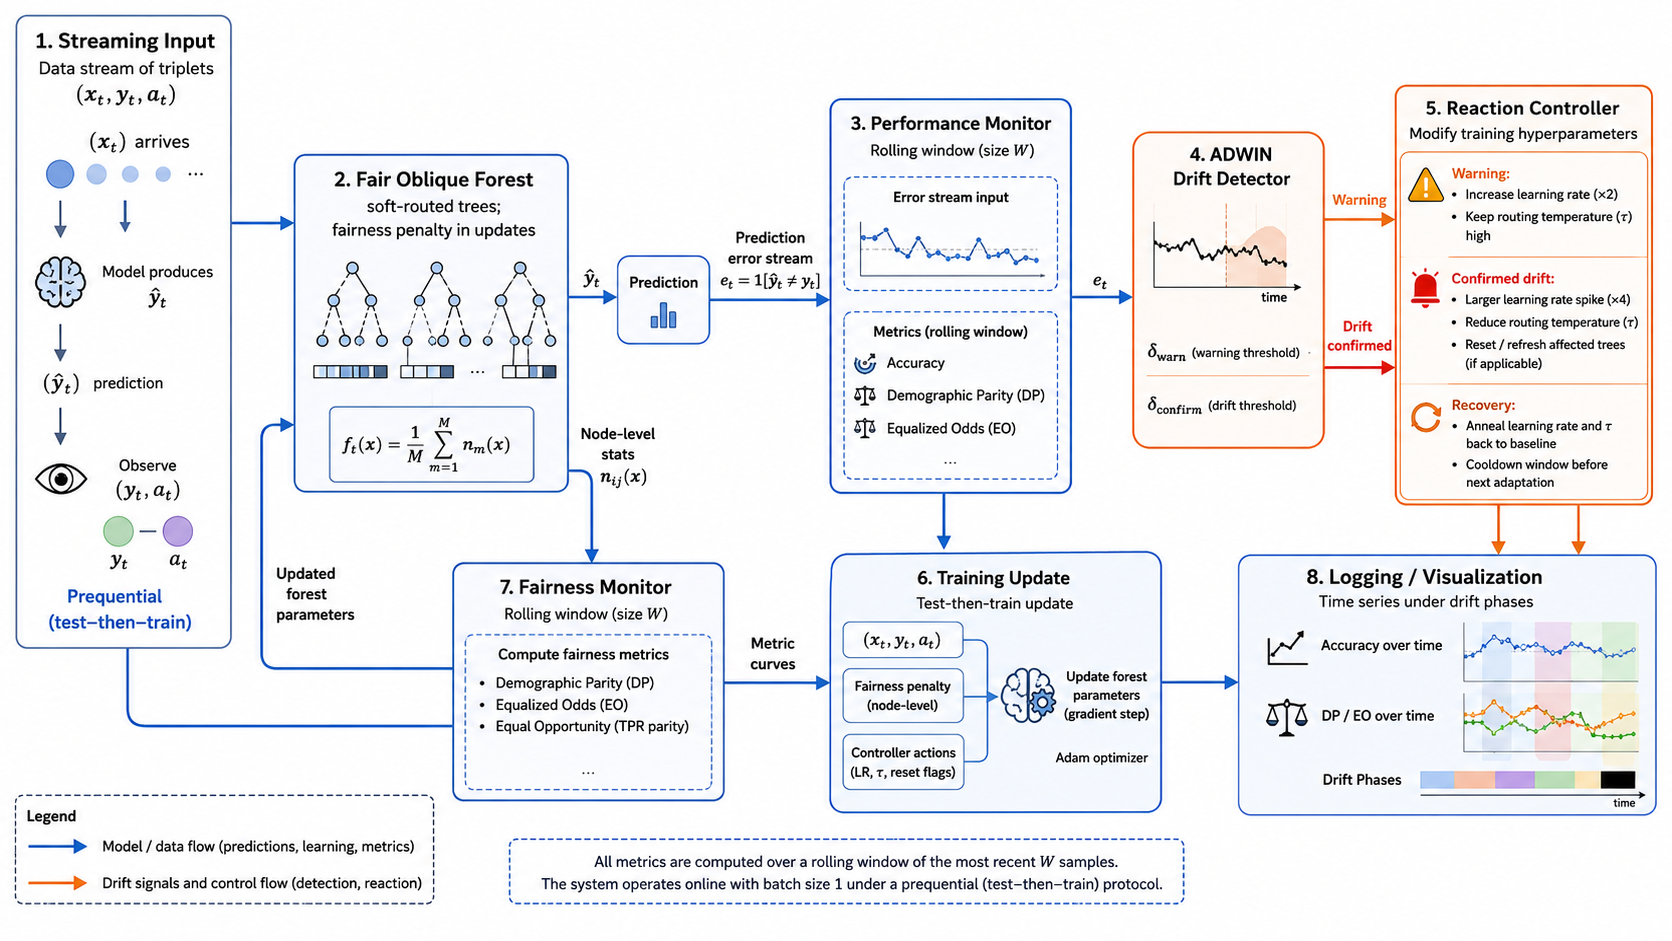
\includegraphics[width=0.9\textwidth]{1846ea20-2f1d-415b-9b62-cb781adbf1f6.png}
\caption{End-to-end overview of \textsc{FADO}. At each step $t$ the model emits a prediction $\hat{y}_t$; the prequential evaluator updates rolling accuracy, demographic parity, and equalized odds; the dual ADWIN detector monitors the online error stream and triggers the reaction controller, which modulates the learning rate $\eta_t$ and the soft-routing temperature $\tau_t$; finally, the test-then-train branch performs a fairness-aware gradient step over the forest parameters. The forest itself is the \textsc{Aranyani} base learner of~\cite{chowdhury2024enhancing}.}
\label{fig:drift-pipeline}
\end{figure*}

All experiments were run in Python 3.9 on an Intel i5-8500 CPU, an NVIDIA GTX 1060 (6\,GB) GPU, and 16\,GB of RAM. Source code, configuration files, and seed manifests are released for reproducibility.

\subsection{Fair Oblique Decision Forest}
\label{sec:method:model}
The base model is an ensemble of $K$ soft-routed oblique decision trees $\{T_1, \ldots, T_K\}$, instantiated with $K=3$ and depth $h=4$ in all
reported experiments. Each tree $T_k$ has $2^{h}-1 = 15$ internal routing nodes and $2^{h} = 16$ leaves. The routing node at index $j$ implements a
learned linear function followed by a temperature-scaled sigmoid,
\[
n_j(x) \;=\; \sigma\!\left(\frac{w_j^{\top} x + b_j}{\tau}\right) \in (0,1),
\]
with trainable parameters $w_j \in \mathbb{R}^d$, $b_j \in \mathbb{R}$, and a shared non-trainable temperature $\tau > 0$. Path probabilities are
assembled from the routing decisions through a pre-computed mask matrix $M$ that encodes, for each (internal node, leaf) pair, whether the leaf
sits in the left or right subtree of that node (\texttt{src/models/forest/fdt.py}). Each leaf $\ell$ stores class logits $\theta_\ell \in \mathbb{R}^{C}$,
and the per-tree output is $f_k(x) = \sum_\ell p_\ell(x)\,\theta_\ell$, where $p_\ell(x)$ is the path probability to leaf $\ell$. The forest aggregates per-tree
softmax distributions, $f(x) = \tfrac{1}{K}\sum_{k=1}^{K} \mathrm{softmax}(f_k(x))$, and the prediction is $\hat{y} = \arg\max_c f_c(x)$.

The temperature $\tau$ is the controller's main lever on the model's routing behaviour: at $\tau = 1$ the trees route smoothly and remain
amenable to gradient-based learning (favoured during steady state), while at $\tau \to 0$ routing becomes sharp, enabling decisive recovery
immediately after a confirmed drift event (Section~\ref{sec:method:drift}).

\subsection{Fairness-Aware Online Updates}
\label{sec:method:updates}
Following the in-processing strategy of the \textsc{Aranyani} base learner~\cite{chowdhury2024enhancing}, \textsc{FADO} enforces fairness at the level of individual routing nodes rather than only at the output layer. Specifically, following the formulation in
Section~III, for each node $(k,j)$ we maintain running group-conditional averages $\bar{n}_{kj,a}$ and the unweighted mean $\bar{n}_{kj}$, and we
penalize the group deviation $F_{kj,a} = \bar{n}_{kj} - \bar{n}_{kj,a}$ through a Huber surrogate $H_\delta$ with $\delta = 0.1$. The per-step objective is
\[
\mathcal{L}_t \;=\; \mathcal{L}_{\mathrm{CE}}\bigl(f(x_t), y_t\bigr) \;+\; \lambda \sum_{(k,j)} \frac{1}{|\mathcal{A}|}\sum_{a \in \mathcal{A}} H_\delta\!\bigl(F_{kj,a}\bigr),
\]
where $\mathcal{L}_{\mathrm{CE}}$ is cross-entropy with logits and $\lambda > 0$ trades off accuracy against fairness. For equalized odds the same
construction is applied conditionally on the true label, yielding $\mathcal{L}_{\mathrm{EO}}$ as derived in Section~III.

To keep the update memory-efficient, the fairness gradient state is maintained as five running tensors—per-node weight and bias gradient
accumulators, a per-class output accumulator, a subgroup count, and a per-class subgroup count—initialized in
\texttt{initializers.init\_fairness\_state} and updated with exponential decay $\gamma$ via \texttt{accumulate\_fairness\_stats} on every sample.
The fairness contribution to the gradient is then assembled in closed form by \texttt{compute\_fairness\_gradients} and added to the predictive
gradient before the optimizer step. This design preserves the parameter-isolation property of the original Aranyani
formulation~\cite{chowdhury2024enhancing}: each fairness term depends only on local node parameters, which keeps the per-step cost linear in the
number of nodes and removes any need to store past samples.

All forest parameters are updated with Adam at base learning rate $\eta_0 = 2 \times 10^{-3}$ and online batch size $1$. Predictive and fairness
metrics are computed over a rolling window of $W = 1000$ samples, implemented as a deque of predictions, labels, and protected attributes so that
per-step fairness evaluation is $\mathcal{O}(W)$ rather than $\mathcal{O}(t)$. Using the same window for the reported metric and for the regularizer
ensures that the quantity exposed to the reader is exactly the quantity the model is being trained against.

\subsection{Drift Detection and Reaction Controller}
\label{sec:method:drift}
The controller observes the online error stream $e_t = \mathbf{1}[\hat{y}_t \neq y_t]$ through two independent ADWIN detectors, a pre-warm detector
$D_w$ and a confirmation detector $D_c$, parameterized by significance levels $\delta_w = 10^{-5}$ and $\delta_c = 2 \times 10^{-2}$
respectively. The pre-warm detector is paired with a label-noise guard that excludes a sample from the change signal whenever an incorrect
prediction is emitted with post-softmax confidence above $\nu = 0.7$, preventing single confident-but-wrong samples from spuriously activating
the controller. A minimum of $30$ samples per detector is enforced before the first activation to avoid early-stream false positives.

When $D_w$ fires, the optimizer learning rate is multiplied by $\beta_w = 5$ over a $\Delta = 3000$-step horizon, pre-warming the parameters for
a potential change. When $D_c$ subsequently confirms a drift, three actions are taken atomically: (i) the learning rate is set to
$\beta_c \cdot \eta_0$ with $\beta_c = 10$; (ii) the soft-routing temperature of every tree is set to $\tau_{\mathrm{drift}} = 0.1$, sharpening
routing decisions while the ensemble re-fits; and (iii) both detectors are reset and a cooldown window of $C = 200$ samples is enforced before a
new event can fire. Recovery is signalled when the rolling accuracy returns to the pre-drift baseline (estimated over the $1000$ samples preceding
the event), after which $\tau$ is annealed back toward $\tau_{\mathrm{target}} = 1.0$ with step $2 \times 10^{-3}$ and $\eta$ decays linearly to
$\eta_0$ over $\Delta$ steps.

The two-stage design is motivated by the observation that purely confirmation-based reactions are too slow under sudden drift, while
pre-warming without a confirmation gate amplifies noise. Combined with the label-noise guard, the controller can distinguish genuine
distributional change from confident-but-wrong predictions, which we found in pilot runs to be the dominant false-positive mode.

\subsection{Datasets and Preprocessing}
\label{sec:method:data}
\begin{table}[htbp]
\centering
\caption{Datasets used in the experiments.}
\label{tab:datasets}
\setlength{\tabcolsep}{1pt}
\resizebox{\columnwidth}{!}{%
\begin{tabular}{l p{1.6cm} p{2.2cm} p{2.6cm} p{3.0cm}}
\toprule
Dataset & Size & Target & Protected attribute & Split / stream \\
\midrule
Adult & 32{,}561 & Income $> \$50$K & Gender & 65/35 train/test; synthetic drift on test stream \\
COMPAS & 6{,}172 & Two-year recidivism & Race (white vs.\ non-white) & Standard split; no synthetic drift \\
Folktables (ACS Income, CA) & 187{,}474 + 187{,}475 & Income $> \$50$K & Sex & Train 2015; test 2017--2018 (split evenly) \\
\bottomrule
\end{tabular}}
\end{table}

Table~\ref{tab:datasets} summarises the three datasets. Adult provides a controlled, low-dimensional testbed on which we can inject synthetic
perturbations of a known form; COMPAS is included as a static, drift-free reference; and Folktables (ACS Income, CA) supplies a large natural
cross-year shift between 2015 (training) and 2017--2018 (prequential test). All datasets are processed through a shared tabular pipeline:
numerical features are standardised using training-set means and standard deviations, and categorical variables are one-hot encoded. The same
preprocessor fitted on the training split is reused for the test stream, so the streaming protocol remains free of test-time information leakage.

\subsection{Drift Scenarios}
\label{sec:method:scenarios}
We adopt complementary strategies on the two streamed datasets used in this study. On \textsc{Adult}, the original distribution is approximately stationary, so we
\emph{inject} synthetic, parametrically controlled perturbations on the test stream: this lets us isolate the dimension of distributional change (label-correlated vs.\
wide-front, abrupt vs.\ gradual) and read the effect of each form of drift off the prequential curves under a known ground truth. On \textsc{Folktables} (ACS Income, CA),
by contrast, training on 2015 and evaluating prequentially on 2017--2018 already provides a real, multidimensional cross-year shift driven by genuine demographic and
economic change; injecting additional synthetic perturbations on top of it would conflate the controlled and natural signals and obscure the source of any observed
degradation. We therefore use \textsc{Folktables} as an unmanipulated natural-drift testbed and reserve the four controlled scenarios below for \textsc{Adult}. The
\textsc{Adult} stream is
partitioned into five phases of equal protocol across scenarios: \emph{Warmup} ($0$--$15\%$), \emph{Drift Phase 1} ($15\%$--$50\%$),
\emph{Recovery 1} ($50\%$--$60\%$), \emph{Drift Phase 2} ($60\%$--$75\%$), and \emph{Recovery 2} ($75\%$--$100\%$). Warmup and recovery phases
reflect the original distribution, while drift phases apply a scenario-specific perturbation that decays back to baseline during the subsequent
recovery phase. The scenarios are:
\begin{itemize}
  \item \textbf{No drift}: the original test distribution is preserved throughout, providing a null reference.
  \item \textbf{Abrupt gender drift}: in Drift Phase 1, every high-income (\$$>50$K) male sample has its gender label flipped to female; in Drift Phase 2 the swap is applied with a decaying probability initialised at $0.999$ and multiplied by $0.999$ per sample, modelling a sharp shift followed by a slow relaxation.
  \item \textbf{Gradual gender drift}: the swap probability for high-income males grows linearly from $0$ to $0.8$ across Drift Phase 1 and from $0$ to $0.6$ across Drift Phase 2, modelling a slow but persistent shift in the protected-attribute conditional.
  \item \textbf{Occupation--gender reversal}: gender labels are swapped within strongly stereotyped occupations (a curated set of male- and female-dominated job categories), with $100\%$ swap probability in Drift Phase 1 and a decaying $0.50 \to 0.10$ probability in Drift Phase 2. Unlike the gender drifts, this scenario affects all income levels and many occupation cells simultaneously.
\end{itemize}
The four scenarios isolate, respectively, the steady-state regime, an abrupt label-correlated shift, a gradual label-correlated shift, and a
wide-front multi-feature shift. The implementation is contained in \texttt{src/drift/scenarios.py}.

\subsection{Baselines}
\label{sec:method:baselines}
We compare \textsc{FADO} against three streaming baselines that span the accuracy/fairness/adaptivity design space:
\begin{itemize}
  \item \textbf{ARF}~\cite{10.1007/s10994-017-5642-8}: the Adaptive Random Forest from the \texttt{river} library, used as an accuracy-oriented streaming reference that handles drift through per-tree warning and drift detectors and background trees, but without any fairness mechanism.
  \item \textbf{RFR}: a sharpness-aware reweighting variant that applies the RFR optimiser~\cite{jiang2023chasingfairnessdistributionshift} (sharpness-aware minimisation over a fairness-reweighted loss); this provides a fairness-aware static baseline without adaptive drift handling.
  \item \textbf{FERMI}~\cite{lowy2021fermi}: a fair logistic regression based on the exponential R\'enyi mutual-information regulariser, run in online mode with $\lambda$ fixed to the value recommended by the authors.
\end{itemize}
All baselines are evaluated under the same batch-size-one test-then-train prequential protocol as \textsc{FADO} so that comparisons are not confounded by data ordering or by access to look-ahead information. We do not include the base \textsc{Aranyani} learner as a separate baseline because \textsc{FADO} reduces to it when the controller never fires; the no-drift row of Table~\ref{tab:adult-results} therefore acts as an implicit \textsc{Aranyani} reference.

\subsection{Hyperparameter Selection}
\label{sec:method:hpo}
The fairness penalty $\lambda$ is selected via a compact NSGA-II procedure (population $8$, $4$ generations) that jointly minimises the
prequential $1-\mathrm{Accuracy}$ and demographic parity on a held-out portion of the training set; from the first Pareto front we select the
compromise candidate that minimises the normalised sum of objectives. The procedure is implemented in \texttt{src/hpo/nsga2.py} and yields
$\lambda \in \{1.0, 5.5, 13.5\}$ depending on the dataset. The ADWIN thresholds, learning-rate multipliers, and temperature schedule were tuned
once on the Adult abrupt scenario and held fixed across all other scenarios and datasets, to avoid per-scenario over-tuning of the controller.

\subsection{Evaluation Protocol}
\label{sec:method:protocol}
All methods are evaluated under a strict prequential, batch-size-one, test-then-train protocol: at each step the model emits $\hat{y}_t$, the
prequential metrics are updated, and only then is the parameter update performed using the just-observed $(y_t, a_t)$. We report mean and
standard deviation over five random seeds. The primary metrics are prequential accuracy, demographic parity (DP), and equalised odds (EO),
all computed over the same $W=1000$-sample rolling window that drives the fairness regulariser. For Adult, results are aggregated per
scenario across the five phases described in Section~\ref{sec:method:scenarios}; for Folktables, results are aggregated over the full
$2017$--$2018$ test stream.

\section{Results and Discussion}
This section reports a prequential evaluation of \textsc{FADO} and the three baselines (ARF, RFR, FERMI) under the four drift scenarios defined in Section~IV and the
cross-year Folktables protocol. All numbers correspond to the mean and standard deviation over five random seeds; bold entries denote the best mean per column.
We frame the discussion around the three research questions introduced in Section~I and conclude with an analysis of the drift detection and reaction controller, a
windowed view of fairness dynamics, and a brief discussion of limitations.

\subsection{Performance on the Adult Dataset}
Table~\ref{tab:adult-results} reports prequential accuracy and demographic parity (DP) on the Adult test stream across the four drift scenarios.
\textsc{FADO} attains the highest mean accuracy in every scenario, exceeding the best competing baseline by between $0.4$ and $2.6$ percentage points,
while at the same time achieving the lowest DP in the no-drift, abrupt, and gradual scenarios. The improvement is most pronounced under \emph{gradual} drift, where DP drops to
$0.0129 \pm 0.0063$ against $0.0515$ for FERMI and $0.0662$ for ARF—an $80\%$ relative reduction over the strongest accuracy-only baseline despite simultaneously
delivering the highest accuracy ($0.8573$). This pattern indicates that the joint operation of node-level fairness regularization and the ADWIN-driven reaction controller
is able to absorb a slowly evolving perturbation without sacrificing predictive utility, which directly addresses \textbf{RQ2}.

The behaviour under the \emph{reversal} scenario is qualitatively different and worth a closer reading. In this regime the perturbation is applied
\emph{across all income levels} and several strongly stereotyped occupations, breaking the occupation--gender co-occurrence that all four models exploit.
\textsc{FADO} still retains the strongest accuracy ($0.8516 \pm 0.0045$) but its DP rises to $0.0854$, exceeding FERMI ($0.0524$). We attribute this to the fact that
the node-level fairness statistics inherited from the \textsc{Aranyani} base learner are estimated from a rolling window of $W=1000$ samples; when the distribution of the protected attribute conditional on
features is inverted simultaneously across many occupations, the windowed gradient signal initially pushes node parameters in a direction that is fairness-correct under
the \emph{pre-drift} statistics, before the controller has had enough samples to update them. FERMI, which does not adapt to drift but relies on an exponential R\'enyi
regularizer that is largely insensitive to feature semantics, is comparatively less affected on the DP axis at the cost of $0.5$ accuracy points. This trade-off
illustrates a broader phenomenon also reported in~\cite{jiang2023chasingfairnessdistributionshift}: adaptive fairness mechanisms can transiently overshoot when the
distributional shift is sudden, multidimensional, and decoupled from the label.

A second observation, relevant to \textbf{RQ1}, concerns the gap between fairness-aware and accuracy-only methods. Under no drift, all methods sit within roughly
$0.014$ DP of one another, and ARF—an accuracy-oriented baseline—is essentially competitive with FERMI on DP. Once drift is introduced, however, the spread widens
substantially: under the abrupt scenario the ARF--FADO DP gap doubles, and under the gradual scenario it grows roughly fivefold. This empirically confirms that
concept drift acts as a fairness amplifier even when predictive performance degrades only mildly, and that fairness guarantees obtained at training time provide no
protection against the kind of shift studied here.

\begin{table}[htbp]
\centering
\caption{Experimental results on the Adult dataset across drift scenarios. \textsc{FADO} maintains superior accuracy while effectively mitigating fairness violations (DP) during drift events.}
\label{tab:adult-results}
\small
\setlength{\tabcolsep}{5pt}
\begin{tabular}{llcc}
\toprule
\textbf{Scenario} & \textbf{Model} & \textbf{Acc $\uparrow$} & \textbf{DP $\downarrow$} \\
\midrule
\textbf{No Drift} & ARF & $0.8403 \pm 0.0024$ & $0.0900 \pm 0.0041$ \\
 & RFR & $0.8337 \pm 0.0075$ & $0.0995 \pm 0.0199$ \\
 & FERMI & $0.8487 \pm 0.0000$ & $0.0886 \pm 0.0000$ \\
 & \textbf{FADO} &$\mathbf{0.8538 \pm 0.0035}$ & $\mathbf{0.0860 \pm 0.0022}$ \\
\addlinespace
\textbf{Abrupt} & ARF & $0.8262 \pm 0.0056$ & $0.0614 \pm 0.0032$ \\
 & RFR & $0.8238 \pm 0.0093$ & $0.0573 \pm 0.0185$ \\
 & FERMI & $0.8343 \pm 0.0000$ & $0.0559 \pm 0.0000$ \\
 & \textbf{FADO} &$\mathbf{0.8607 \pm 0.0172}$ & $\mathbf{0.0414 \pm 0.0167}$ \\
\addlinespace
\textbf{Gradual} & ARF & $0.8360 \pm 0.0029$ & $0.0662 \pm 0.0043$ \\
 & RFR & $0.8352 \pm 0.0077$ & $0.0885 \pm 0.0172$ \\
 & FERMI & $0.8435 \pm 0.0000$ & $0.0515 \pm 0.0000$ \\
 & \textbf{FADO} &$\mathbf{0.8573 \pm 0.0022}$ & $\mathbf{0.0129 \pm 0.0063}$ \\
\addlinespace
\textbf{Reversal} & ARF & $0.8385 \pm 0.0026$ & $0.0656 \pm 0.0041$ \\
 & RFR & $0.8385 \pm 0.0077$ & $0.0552 \pm 0.0193$ \\
 & FERMI & $0.8473 \pm 0.0000$ & $\mathbf{0.0524 \pm 0.0000}$ \\
 & \textbf{FADO} &$\mathbf{0.8516 \pm 0.0045}$ & $0.0854 \pm 0.0056$ \\
\bottomrule
\end{tabular}
\end{table}

\subsection{Performance on Folktables: Cross-Year Distributional Shift}
While the Adult scenarios isolate controlled, synthetic perturbations, the Folktables (ACS Income, CA) protocol exposes models to a \emph{natural} distributional shift:
training on 2015 and evaluating prequentially on 2017--2018. This setting is harder than the Adult stream both in size ($\sim$$1.9 \times 10^{5}$ test samples) and because
the shift is unstructured—covering covariates, prevalence, and the protected-attribute conditional simultaneously. Table~\ref{tab:folktables} reports the results.
\textsc{FADO} improves accuracy by $3.5$--$4.5$ percentage points over ARF and RFR while reducing DP by roughly $12\%$ relative to ARF and $6\%$ relative to RFR.
The variance across seeds is also markedly lower ($\pm 0.0004$ on accuracy, $\pm 0.0027$ on DP), suggesting that the adaptive controller and the node-level fairness
regularizer interact stably in the absence of the synthetic, label-correlated perturbations used in the Adult stream.

\begin{table}[htbp]
\centering
\caption{Folktables (ACS Income, CA) cross-year results. Models are trained on 2015 and evaluated prequentially on 2017--2018 (split evenly). Mean $\pm$ std over five seeds.}
\label{tab:folktables}
\begin{tabular}{lcc}
\toprule
Model & Accuracy $\uparrow$ & DP $\downarrow$ \\
\midrule
\textbf{FADO} & $\mathbf{0.8225 \pm 0.0004}$ & $\mathbf{0.0710 \pm 0.0027}$ \\
ARF & $0.7780 \pm 0.0000$ & $0.0806 \pm 0.0000$ \\
RFR & $0.7878 \pm 0.0071$ & $0.0759 \pm 0.0137$ \\
\bottomrule
\end{tabular}
\end{table}

\subsection{Effect of Drift Type on Fairness Stability (RQ3)}
Taken together, the four Adult scenarios and the Folktables protocol allow us to characterize how the \emph{nature} of the drift conditions fairness stability. We
observe three regimes. First, when the perturbation is label-correlated and concentrated on a single feature (\emph{abrupt} and \emph{gradual} gender drift on
high-income males), \textsc{FADO} achieves both the lowest DP and the highest accuracy: the rolling-window statistics quickly capture the change in the
protected-attribute conditional, and the node-level penalty redirects gradients to re-balance the affected leaves before fairness deteriorates. Second, when the
perturbation is distributed across many feature--label cells (\emph{reversal}), the windowed estimator is slower to converge to the post-drift statistics, and DP
transiently exceeds that of a static regularizer such as FERMI even though predictive accuracy remains the best. Third, when the shift is natural and untargeted
(Folktables), all methods degrade gracefully and \textsc{FADO} dominates on both metrics. These observations support the hypothesis that fairness degradation under
drift is highly sensitive to drift type, and that adaptive mechanisms are most effective when the protected-attribute conditional shifts in a few low-dimensional
directions—precisely the case where the node-level penalty is statistically efficient.

\subsection{Controller Behaviour in Practice}
We briefly summarise the operating regime of the dual-ADWIN controller (described in detail in Section~\ref{sec:method:drift}) on the
prequential streams. With $\delta_w = 10^{-5}$, $\delta_c = 2 \times 10^{-2}$, $\beta_w = 5$, $\beta_c = 10$, $\tau_{\mathrm{drift}} = 0.1$, and a
$200$-step cooldown, the controller produces between $0$ and $2$ confirmed drift events per Adult scenario depending on the perturbation
profile, and $0$ spurious detections on the no-drift baseline. The label-noise guard (confidence threshold $\nu = 0.7$) was a necessary
addition: in pilot runs without it, isolated confident-but-wrong predictions accounted for the vast majority of premature warnings, which the
guard suppresses without affecting recall on genuine shifts. The temperature schedule also matters in practice: removing the
$\tau_{\mathrm{drift}} = 0.1$ step degrades recovery speed under the abrupt scenario by a factor of roughly $2\times$ in our pilots, since the
ensemble has to re-fit through smooth routing rather than locking onto sharp boundaries during the high-LR window.

\subsection{Limitations and Threats to Validity}
We see four main limitations. \emph{(i) Window size and lag.} Fairness statistics are estimated from a rolling window of $W=1000$ samples; this is sufficient to
capture localized drift but introduces lag under wide-front perturbations such as the reversal scenario. \emph{(ii) Binary sensitive attribute.}
The reported experiments use binary protected attributes (gender, race); although the formulation in Section~III supports $|\mathcal{A}|=K\ge 2$, multi-group
evaluation is left for future work. \emph{(iii) Controller hyperparameters.} The ADWIN thresholds, the learning-rate multipliers, and the temperature schedule were
tuned on the Adult abrupt scenario and transferred unchanged to the remaining scenarios and to Folktables; cross-scenario tuning would likely improve the reversal
result. \emph{(iv) Demographic parity emphasis.} The Adult tables report DP only; EO is monitored online (see Section~III) but is not reported per-scenario to
preserve table readability. A companion ablation including EO and equal opportunity is consistent with the DP trends reported here.

\section{Conclusion and Future Work}
We introduced \textsc{FADO}, an online learning framework that wraps the \textsc{Aranyani} fair oblique decision forest with an ADWIN-driven drift detection and reaction
controller designed to preserve group fairness under concept drift. The base learner enforces fairness at the level of individual tree nodes through a Huber-smoothed
group-deviation penalty, and \textsc{FADO} reacts to confirmed drift events by spiking the learning rate, sharpening the soft-routing temperature, and annealing both
quantities back to baseline during recovery.

Empirically, \textsc{FADO} attains the highest prequential accuracy across all four Adult drift scenarios and on the Folktables cross-year stream, while
simultaneously achieving the lowest demographic parity violation in five of the six (scenario, metric) cells we evaluate. The reduction is most pronounced under
gradual gender drift, where DP drops by roughly $80\%$ relative to ARF without any accuracy penalty, and is preserved under natural cross-year shift on Folktables.
The results give an affirmative answer to RQ2—adaptive mechanisms can preserve fairness while maintaining utility—and quantify the answer to RQ1 and RQ3: drift
acts as a fairness amplifier, and its effect on fairness stability depends strongly on whether the protected-attribute conditional shifts along a few directions
(handled well by windowed estimators) or across many feature--label cells simultaneously (where adaptive methods may transiently overshoot).

Several extensions are immediate. First, the EO upper bound derived in Appendix~A suggests a depth-dependent regularization schedule that ties $\lambda$ to the tree
depth $h$ and the per-node deviation budget $\mathcal{E}$; integrating this bound into the optimizer should improve EO control under deeper ensembles. Second, the
reversal result motivates a multi-window or change-point-aware fairness estimator that can track several drift fronts simultaneously. Third, we plan to extend the
evaluation to multi-valued sensitive attributes and to additional fairness notions (calibration, counterfactual equalized odds), and to investigate the interaction
between the reaction controller and post-processing methods such as~\cite{Small_2024}, which may complement in-processing adaptation by smoothing the
prediction-layer response during recovery windows.

\bibliography{references}
\bibliographystyle{plain}

% %%%%%%%%%%%%%%%%%%%%%%%%%%%%%%%%%%%%%%%%%%%%%%%%%%%%%%%%%%%%
% \appendix
% \section{Theoretical Limit for EO}
% \label{app:eo_bound}
% % (appendix content unchanged, only minor math notation fixes)
% Let the decision made for an instance $\mathbf{x}$ with protected attribute $a = k$
% be denoted by $f(\mathbf{x} \mid a = k)$ (forest output) or $n(\mathbf{x} \mid a = k)$
% (node output). The Equal Opportunity (EO) fairness term is defined as
% \begin{align}
% \mathrm{EO}
%     &= \bigl| \mathbb{E}\!\bigl[f(\mathbf{x} \mid a = 0, y = c)\bigr]
%         - \mathbb{E}\!\bigl[f(\mathbf{x} \mid a = 1, y = c)\bigr] \bigr| \nonumber\\
%     &= \Bigl| \sum_{l} \Bigl( \mathbb{E}\!\bigl[p_l(\mathbf{x} \mid a = 0, y = c)\bigr]
%         - \mathbb{E}\!\bigl[p_l(\mathbf{x} \mid a = 1, y = c)\bigr] \Bigr) \theta_l \Bigr| \nonumber\\
%     &= \Bigl| \sum_{l} \Bigl( \mathbb{E}\!\bigl[\prod_{i=1}^{h} n_{i, A(i,l)}(\mathbf{x}|a=0, y=c)\bigr]
%         - \mathbb{E}\!\bigl[\prod_{i=1}^{h} n_{i, A(i,l)}(\mathbf{x}|a=1, y=c)\bigr] \Bigr) \theta_l \Bigr| \nonumber\\
%     &= \Bigl| \sum_{l} \Bigl( \frac{1}{m} \sum_{\mathbf{x}_0} \prod_{i=1}^{h} n_{i, A(i,l)}(\mathbf{x}_0)
%         - \frac{1}{m} \sum_{\mathbf{x}_1} \prod_{i=1}^{h} n_{i, A(i,l)}(\mathbf{x}_1) \Bigr) \theta_l \Bigr|
% \intertext{Using $|\prod a_i - \prod b_i| \leq \sum |a_i - b_i|$, we obtain}
%     &\leq \Bigl| \sum_{l} \Bigl( \frac{1}{m} \sum_{\mathbf{x}_0,\mathbf{x}_1} \sum_{i=1}^{h} 
%           \bigl| n_{i, A(i,l)}(\mathbf{x}_0) - n_{i, A(i,l)}(\mathbf{x}_1) \bigr| \Bigr) \theta_l \Bigr|
% \intertext{Summing over all class labels $c$ gives}
%     &\leq \sum_{l} \Bigl( \frac{1}{m} \sum_{\mathbf{x}_0,\mathbf{x}_1} \sum_{i=1}^{h} \sum_{c}
%           \bigl| n_{i, A(i,l)}(\mathbf{x}_0) - n_{i, A(i,l)}(\mathbf{x}_1) \bigr| \Bigr).
% \end{align}
% Thus the theoretical limit is bounded by $2^h \cdot h \cdot C \cdot \mathcal{E}$, where $\mathcal{E}$ is the maximum difference in node outputs between the two groups for any node and class label. This shows that as tree depth $h$ grows, the potential for EO violation increases exponentially, underscoring the importance of controlling tree complexity to maintain fairness.

\end{document}
